%-----------------------------------------------------------------------------%
\chapter{ANALISIS DAN PERANCANGAN SISTEM}
%-----------------------------------------------------------------------------%
\vspace{4.5pt}

\section{Analisis Masalah}
Arsitektur yang digunakan Odoo(ERP) masih beruba monolith sehingga memiliki kelemahan seperti skalabilitas, sulit dikembangkan berkelanjutan, dan terkunci pada teknologi tertentu.
Arsitektur Microservice dapat menyelesaikan masalah tersebut
Namun diperlukan proses dekomposisi dari mono-to-micro. Proses dekomposisi sendiri  tidak mudah dan melelahkan karena masih membutuhkan proses manual. 
Proses manual ini bisa di”mudahkan” dengan melakukan clustering khususnya dengan metode hierarchical 
Sebelum melakukan proses clustering diperlukan analisis kode seperti Call Graph untuk mendapatkan graph dari source code aplikasi Odoo (ERP)
Hasil terbaik dari clustering diimplementasikan menjadi service, service dan dilakukan pemecahan dengan pattern yang sudah ditemukan
Dilakukan evaluasi dari aplikasi yang dibangun untuk menentukan apakah microservice dan clustering bisa melakukan dekomposisi dapat menyelesaikan permasalahan pada kasus ERP

\section{Kerangka Pemikiran}
\begin{center}
	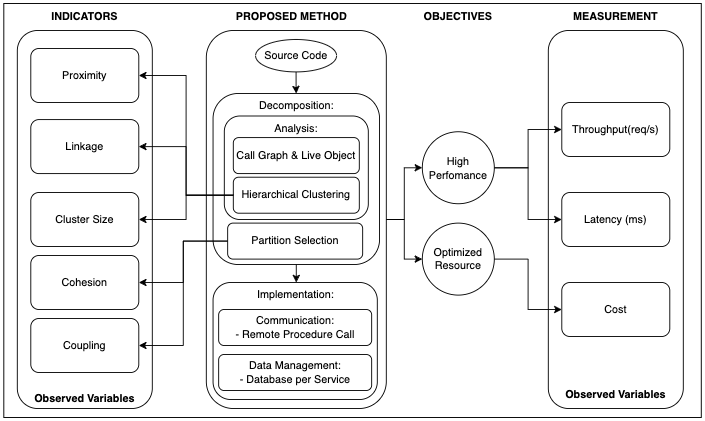
\includegraphics[width=14cm]{img/KerangkaPemikiran.png}
	\captionof{figure}{Kerangka Pemikiran}
	\label{fig:asd}
\end{center}

Penelitian akan dimulai dengan menggunakan kode sumber aplikasi yang dibuat dengan monolit. Kode sumber ini dilakukan proses dekomposisi yaitu dengan analisis seperti mencari objek beserta atributnya, untuk mencari keterhubungan lebih lanjut tentang objek maka dilakukan pencarian pada fungsi-fungsi sehingga terbentuklah grafik yang menunjukan bagaimana keterhubungan objek di aplikasi.

Dari grafik yang sudah dibuat akan dilakukan pengelompokan dengan pendekatan Hierarchical Clustering. Dimana perlu ditentukan jumlah cluster minimum yang harus ditemukan dan pemilihan algoritma Linkage. Metode linkage yaitu menentukan jarak atau kemiripan antara semua objek. Untuk menentukan jarak ini bisa dengan rata-rata, maximum, minimum dan mengecilkan variance.

Pengelompokan dari Hierarchical Clustering akan dipilih dengan mencari nilai cohesion terendah dan  nilai coupling tertinggi. Dimana Internal Coupling mengevaluasi tingkat ketergantungan langsung dan tidak langsung antar objek. Semakin banyak dua objek menggunakan metode masing-masing semakin mereka menjadi satu kesatuan. Sedangkan Internal Cohesion akan mengevaluasi kekuatan interaksi antar objek. Biasanya, dua objek atau lebih menjadi interaktif jika metodenya bekerja pada atribut yang sama.

Ketika analisis dekomposisi sudah selesai dilakukan maka akan dilakukan implementasi berdasarkan pengelompokannya masing-masing yang akan menjadi service. Untuk metode komunikasinya antara service yaitu dengan Remote Procedure Call(RPC) dan untuk mengelola data, setiap service memiliki databasenya masing-masing dan untuk menjaga konsistensi data antar service maka digunakan pendekatan SAGA dengan cara choreography.

Untuk mengetahui bagaimana performa dari microservice dibandingkan dengan monolit yaitu dengan test beban. Pengukuran performa dilihat dari throughput, jumlah response, dan latency. 


\section{Urutan Proses Global}
\begin{center}
	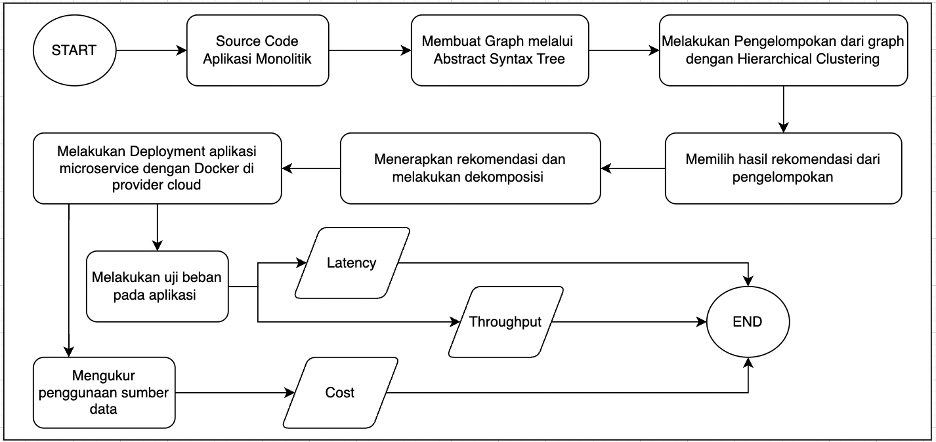
\includegraphics[width=14cm]{img/FlowchartProsesGlobal.png}
	\captionof{figure}{Diagram Flowchart Proses Global }
	\label{fig:asd}
\end{center}

\subsection{Proses Clustering}
3.X.X Flowchart Proses Clustering
\begin{enumerate}
  \item Pengambilan Source Code
Mengunduh dari branch main/master terbaru dan semua test workflow pass
\item Pembuatan Call Graph
Menggunakan library call graph (pycg atau pycallgraph)
\item Ilustrasi Graph
Ilustrasi menggunakan tools graphviz
\item Extrasi Call Graph
Proses ekstraksi json 
\item Pengelompokan dari graph
Menggunakan python dan library hirarki clustering 
Memilih hasil rekomendasi \\
\end{enumerate}

\subsection{Dekomposisi Monolitik ke Microservice}
Komponen Diagram monolith VS komponen diagram yang diolah dari call graph\\
Sequence Diagram antar service dan module

\subsection{Deployment}
\begin{center}
	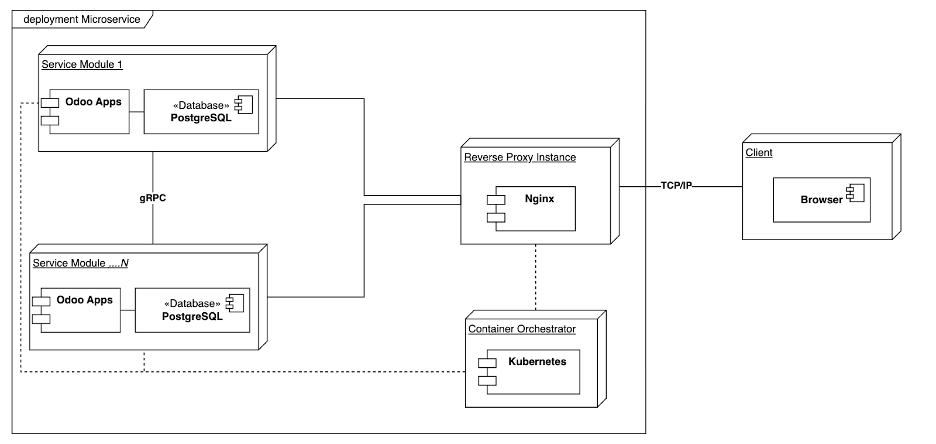
\includegraphics[width=14cm]{img/Deployment.png}
	\captionof{figure}{Diagram Deployment }
	\label{fig:asd}
\end{center}

\subsection{Evaluasi}
Latency \& Throughput:  JMeter\\
Cost: AWS Cost Management (Cost Explorer)
